%%%%%%%%%%%%%%%%%%%%%%%%%%%%%%%%%%%%%%%%%
% Lachaise Assignment
% LaTeX Template
% Version 1.0 (26/6/2018)
%
% This template originates from:
% http://www.LaTeXTemplates.com
%
% Authors:
% Marion Lachaise & François Févotte
% Vel (vel@LaTeXTemplates.com)
%
% License:
% CC BY-NC-SA 3.0 (http://creativecommons.org/licenses/by-nc-sa/3.0/)
% 
%%%%%%%%%%%%%%%%%%%%%%%%%%%%%%%%%%%%%%%%%


%----------------------------------------------------------------------------------------
%    PACKAGES AND OTHER DOCUMENT CONFIGURATIONS
%----------------------------------------------------------------------------------------

\documentclass[11pt]{article}

%%%%%%%%%%%%%%%%%%%%%%%%%%%%%%%%%%%%%%%%%
% Lachaise Assignment
% Structure Specification File
% Version 1.0 (26/6/2018)
%
% This template originates from:
% http://www.LaTeXTemplates.com
%
% Authors:
% Marion Lachaise & François Févotte
% Vel (vel@LaTeXTemplates.com)
%
% License:
% CC BY-NC-SA 3.0 (http://creativecommons.org/licenses/by-nc-sa/3.0/)
% 
%%%%%%%%%%%%%%%%%%%%%%%%%%%%%%%%%%%%%%%%%

%----------------------------------------------------------------------------------------
%    PACKAGES AND OTHER DOCUMENT CONFIGURATIONS
%----------------------------------------------------------------------------------------

\usepackage{amsmath,amsfonts,stmaryrd,amssymb} % Math packages
\usepackage{xfrac, dsfont}

\usepackage{enumerate} % Custom item numbers for enumerations

\usepackage[ruled]{algorithm2e} % Algorithms

\usepackage[framemethod=tikz]{mdframed} % Allows defining custom boxed/framed environments

\usepackage{listings} % File listings, with syntax highlighting
\lstset{
    basicstyle=\ttfamily, % Typeset listings in monospace font
}

\usepackage[
    colorlinks=true,
    linkcolor=black
]{hyperref}
\usepackage{bookmark}   % bookmarks for PDF viewing

\numberwithin{equation}{section}

%%Figure and table packages
\usepackage{booktabs,caption}
\usepackage[flushleft]{threeparttable}
\usepackage{graphicx}
\usepackage{float}
\usepackage{tabularx}
\usepackage{multirow}

\usepackage{fancyhdr}	% Header and footer control

\usepackage{minted}	% Code formatting and syntax highlighting
%\surroundwithmdframed{minted}
\definecolor{DarkGray}{rgb}{0.9, 0.9, 0.9}
\setminted{linenos=true,
    autogobble=true,
    breaklines=true, breakautoindent=true,
    bgcolor=DarkGray,
    python3=true,
    frame=lines
}
\setmintedinline{bgcolor=DarkGray}

\usepackage{chngcntr}
\counterwithin{figure}{section}

% Referencing manager
%%\usepackage[
%%	backend=biber,
%%	style=ieee
%%]{biblatex}

%----------------------------------------------------------------------------------------
%    DOCUMENT MARGINS
%----------------------------------------------------------------------------------------

\usepackage{geometry} % Required for adjusting page dimensions and margins

\geometry{
    paper=a4paper, % Paper size, change to letterpaper for US letter size
    top=2.5cm, % Top margin
    bottom=2.5cm, % Bottom margin
    left=2.5cm, % Left margin
    right=2.5cm, % Right margin
    headheight=14pt, % Header height
    footskip=1.5cm, % Space from the bottom margin to the baseline of the footer
    headsep=1.2cm, % Space from the top margin to the baseline of the header
    %showframe, % Uncomment to show how the type block is set on the page
}

%----------------------------------------------------------------------------------------
%    FONTS
%----------------------------------------------------------------------------------------

\usepackage[utf8]{inputenc} % Required for inputting international characters
\usepackage[T1]{fontenc} % Output font encoding for international characters
\linespread{1.3}        % 1.5 line spacing
\usepackage{XCharter} % Use the XCharter fonts
\usepackage[none]{hyphenat} % prevent words being split across multiple lines
\usepackage{url}

% strikethrough within math mode
\newcommand\hcancel[2][black]{\setbox0=\hbox{$#2$}%
\rlap{\raisebox{.45\ht0}{\textcolor{#1}{\rule{\wd0}{1pt}}}}#2}

%----------------------------------------------------------------------------------------
%    COMMAND LINE ENVIRONMENT
%----------------------------------------------------------------------------------------

% Usage:
% \begin{commandline}
%    \begin{verbatim}
%        $ ls
%        
%        Applications    Desktop    ...
%    \end{verbatim}
% \end{commandline}

\mdfdefinestyle{commandline}{
    leftmargin=10pt,
    rightmargin=10pt,
    innerleftmargin=15pt,
    middlelinecolor=black!50!white,
    middlelinewidth=2pt,
    frametitlerule=false,
    backgroundcolor=black!5!white,
    frametitle={Command Line},
    frametitlefont={\normalfont\sffamily\color{white}\hspace{-1em}},
    frametitlebackgroundcolor=black!50!white,
    nobreak,
}

% Define a custom environment for command-line snapshots
\newenvironment{commandline}{
    \medskip
    \begin{mdframed}[style=commandline]
}{
    \end{mdframed}
    \medskip
}

%----------------------------------------------------------------------------------------
%    FILE CONTENTS ENVIRONMENT
%----------------------------------------------------------------------------------------

% Usage:
% \begin{file}[optional filename, defaults to "File"]
%    File contents, for example, with a listings environment
% \end{file}

\mdfdefinestyle{file}{
    innertopmargin=1.6\baselineskip,
    innerbottommargin=0.8\baselineskip,
    topline=false, bottomline=false,
    leftline=false, rightline=false,
    leftmargin=2cm,
    rightmargin=2cm,
    singleextra={%
        \draw[fill=black!10!white](P)++(0,-1.2em)rectangle(P-|O);
        \node[anchor=north west]
        at(P-|O){\ttfamily\mdfilename};
        %
        \def\l{3em}
        \draw(O-|P)++(-\l,0)--++(\l,\l)--(P)--(P-|O)--(O)--cycle;
        \draw(O-|P)++(-\l,0)--++(0,\l)--++(\l,0);
    },
    nobreak,
}

% Define a custom environment for file contents
\newenvironment{file}[1][File]{ % Set the default filename to "File"
    \medskip
    \newcommand{\mdfilename}{#1}
    \begin{mdframed}[style=file]
}{
    \end{mdframed}
    \medskip
}

%----------------------------------------------------------------------------------------
%    NUMBERED QUESTIONS ENVIRONMENT
%----------------------------------------------------------------------------------------

% Usage:
% \begin{question}[optional title]
%    Question contents
% \end{question}

\mdfdefinestyle{question}{
    innertopmargin=1.2\baselineskip,
    innerbottommargin=0.8\baselineskip,
    roundcorner=5pt,
    nobreak,
    singleextra={%
        \draw(P-|O)node[xshift=1em,anchor=west,fill=white,draw,rounded corners=5pt]{%
        Question \theQuestion\questionTitle};
    },
}

\newcounter{Question} % Stores the current question number that gets iterated with each new question

% Define a custom environment for numbered questions
\newenvironment{question}[1][\unskip]{
    \bigskip
    \stepcounter{Question}
    \newcommand{\questionTitle}{~#1}
    \begin{mdframed}[style=question]
}{
    \end{mdframed}
    \medskip
}

%----------------------------------------------------------------------------------------
%    WARNING TEXT ENVIRONMENT
%----------------------------------------------------------------------------------------

% Usage:
% \begin{warn}[optional title, defaults to "Warning:"]
%    Contents
% \end{warn}

\mdfdefinestyle{warning}{
    topline=false, bottomline=false,
    leftline=false, rightline=false,
    nobreak,
    singleextra={%
        \draw(P-|O)++(-0.5em,0)node(tmp1){};
        \draw(P-|O)++(0.5em,0)node(tmp2){};
        \fill[black,rotate around={45:(P-|O)}](tmp1)rectangle(tmp2);
        \node at(P-|O){\color{white}\scriptsize\bf !};
        \draw[very thick](P-|O)++(0,-1em)--(O);%--(O-|P);
    }
}

% Define a custom environment for warning text
\newenvironment{warn}[1][Warning:]{ % Set the default warning to "Warning:"
    \medskip
    \begin{mdframed}[style=warning]
        \noindent{\textbf{#1}}
}{
    \end{mdframed}
}

%----------------------------------------------------------------------------------------
%    INFORMATION ENVIRONMENT
%----------------------------------------------------------------------------------------

% Usage:
% \begin{info}[optional title, defaults to "Info:"]
%     contents
% \end{info}

\mdfdefinestyle{info}{%
    topline=false, bottomline=false,
    leftline=false, rightline=false,
    nobreak,
    singleextra={%
        \fill[black](P-|O)circle[radius=0.4em];
        \node at(P-|O){\color{white}\scriptsize\bf i};
        \draw[very thick](P-|O)++(0,-0.8em)--(O);%--(O-|P);
    }
}

% Define a custom environment for information
\newenvironment{info}[1][Info:]{ % Set the default title to "Info:"
    \medskip
    \begin{mdframed}[style=info]
        \noindent{\textbf{#1}}
}{
    \end{mdframed}
}

\usepackage{XCharter} % Include the file specifying the document structure and custom commands

\usepackage{draftwatermark}
\SetWatermarkText{\textsf{\textbf{CONFIDENTAL}}}
\SetWatermarkScale{2.5}
\SetWatermarkColor[gray]{0.8}
\SetWatermarkAngle{50}

\pagestyle{fancy}
\fancyhf{}
\renewcommand{\headrulewidth}{2pt}
\renewcommand{\footrulewidth}{1pt}
\lhead{\textit{Certificate Maker Kickstart Manual}}
\rhead{\leftmark}
\cfoot{Page \thepage}

%----------------------------------------------------------------------------------------
%    ASSIGNMENT INFORMATION
%----------------------------------------------------------------------------------------

\title{Certificate Maker Kickstart Manual} % Title of the assignment

\author{Harrison Outram\\ Membership Officer}

\date{Curtin IET On Campus --- \today} % University, school and/or department name(s) and a date

%----------------------------------------------------------------------------------------

\begin{document}

%----------------------------------------------------------------------------------------
%    TITLE PAGE
%----------------------------------------------------------------------------------------

\begin{titlepage} % Suppresses displaying the page number on the title page and the subsequent page counts as page 1
    \newcommand{\HRule}{\rule{\linewidth}{0.5mm}} % Defines a new command for horizontal lines, change thickness here
    
    \center % Centre everything on the page
    
    %------------------------------------------------
    %    Headings
    %------------------------------------------------
    
    \textsc{\LARGE Curtin IET On Campus}\\[1.5cm] % Main heading such as the name of your university/college
    
    \textsc{\LARGE Institute of Engineering and Technology}\\[0.5cm] % Major heading such as course name
    
    %------------------------------------------------
    %    Title
    %------------------------------------------------
    
    \HRule\\[0.4cm]

    \vspace{0.4cm}
    
    {\Huge\bfseries Certificate Maker Kickstart Manual}\\[0.4cm] % Title of your document
    
    \HRule\\[1.5cm]
    
    %------------------------------------------------
    %    Author(s)
    %------------------------------------------------
    
    \begin{center}
        \large
        Harrison G. Outram \\
        Membership Officer
    \end{center}
    
    %------------------------------------------------
    %    Date
    %------------------------------------------------
    
    \vfill\vfill\vfill % Position the date 3/4 down the remaining page
    
    {\Large\today} % Date, change the \today to a set date if you want to be precise
    
    %------------------------------------------------
    %    Logo
    %------------------------------------------------
    
    \vfill
    
\includegraphics[width=0.8\textwidth]{../../assets/IET_Logo_Blue_RGB.pdf}\\
     
    %----------------------------------------------------------------------------------------
    
    \vfill % Push the date up 1/4 of the remaining page
    
\end{titlepage}

\pagenumbering{roman}

\tableofcontents

\bigskip

\listoffigures

\newpage

%----------------------------------------------------------------------------------------
%    INTRODUCTION
%----------------------------------------------------------------------------------------

\pagenumbering{arabic}
\setcounter{page}{1}

\section{Introduction}

\subsection{Context}

Curtin IET On Campus (or ``CIET'' for short) provides multiple industry talks and workshops to STEM students (particularly engineering and computer related science). As part of CIET's commitment to quality, attendees shall recieve a certificate of attendance stating the name of the event, the club name, the president's full name with a signature, the the attendee's full name, and the number of approved CPD hours. This certificate of attendance must be done in a PDF document with vector graphics where possible, then emailed to attendees as soon as possible. This is particularly important for undergraduate engineering students, as one graduation requirement is to obtain a minimum of 16 weighted hours (or five and a third actual) in the PRES category (technical presentations and workshops by a professional body). By creating and sending out these certificates, CIET is holding itself to a high standard of attendee satisfaction and professional development.

\subsection{Problem}

Despite the necessity of creating and sending certificates, the process for doing so is extremely time consuming and error prone. As shown in Figure \ref{fig:old-solution}, this process is comprised of four stages: (1) the attendee record must be collected from the events team and checked for errors, e.g. multiple registrations from one person or missing but required information. (2) one certificate is made for each attendee via the template on CIET's Canva account. Each certificate is then checked one by one for errors, being recreated if erroneous. (3) the certificates are uploaded to CIET's MailChimp account, where MailChimp auto-generates a URI for each certificate, required later on. Unfortunately, these URIs involve a randomly generated hexadecimal string, meaning each URI must be recorded manually in the attendee record, then checked for errors. Once the attendee record has been updated with certificate URIs, it is uploaded to MailChimp. (4) The certificates are checked one last time by creating a mock campaign on MailChimp, going through each attendee, downloading the certificate, then checking the certificate for errors and fixing where erroneous. All up, this process takes at least two hours per 50 attendees for someone who has gone through it before, and \textbf{far} longer for someone who has not. Worse yet, despite every certificate being checked three times during this process, it is still possible for erroneous certificates to be sent out, which has happened on at least one occasion. Clearly, this process is extremely time consuming and error prone, leading to attendee frustration and a negative impact on CIET's reputation.

\newpage

\begin{figure}[h!]
    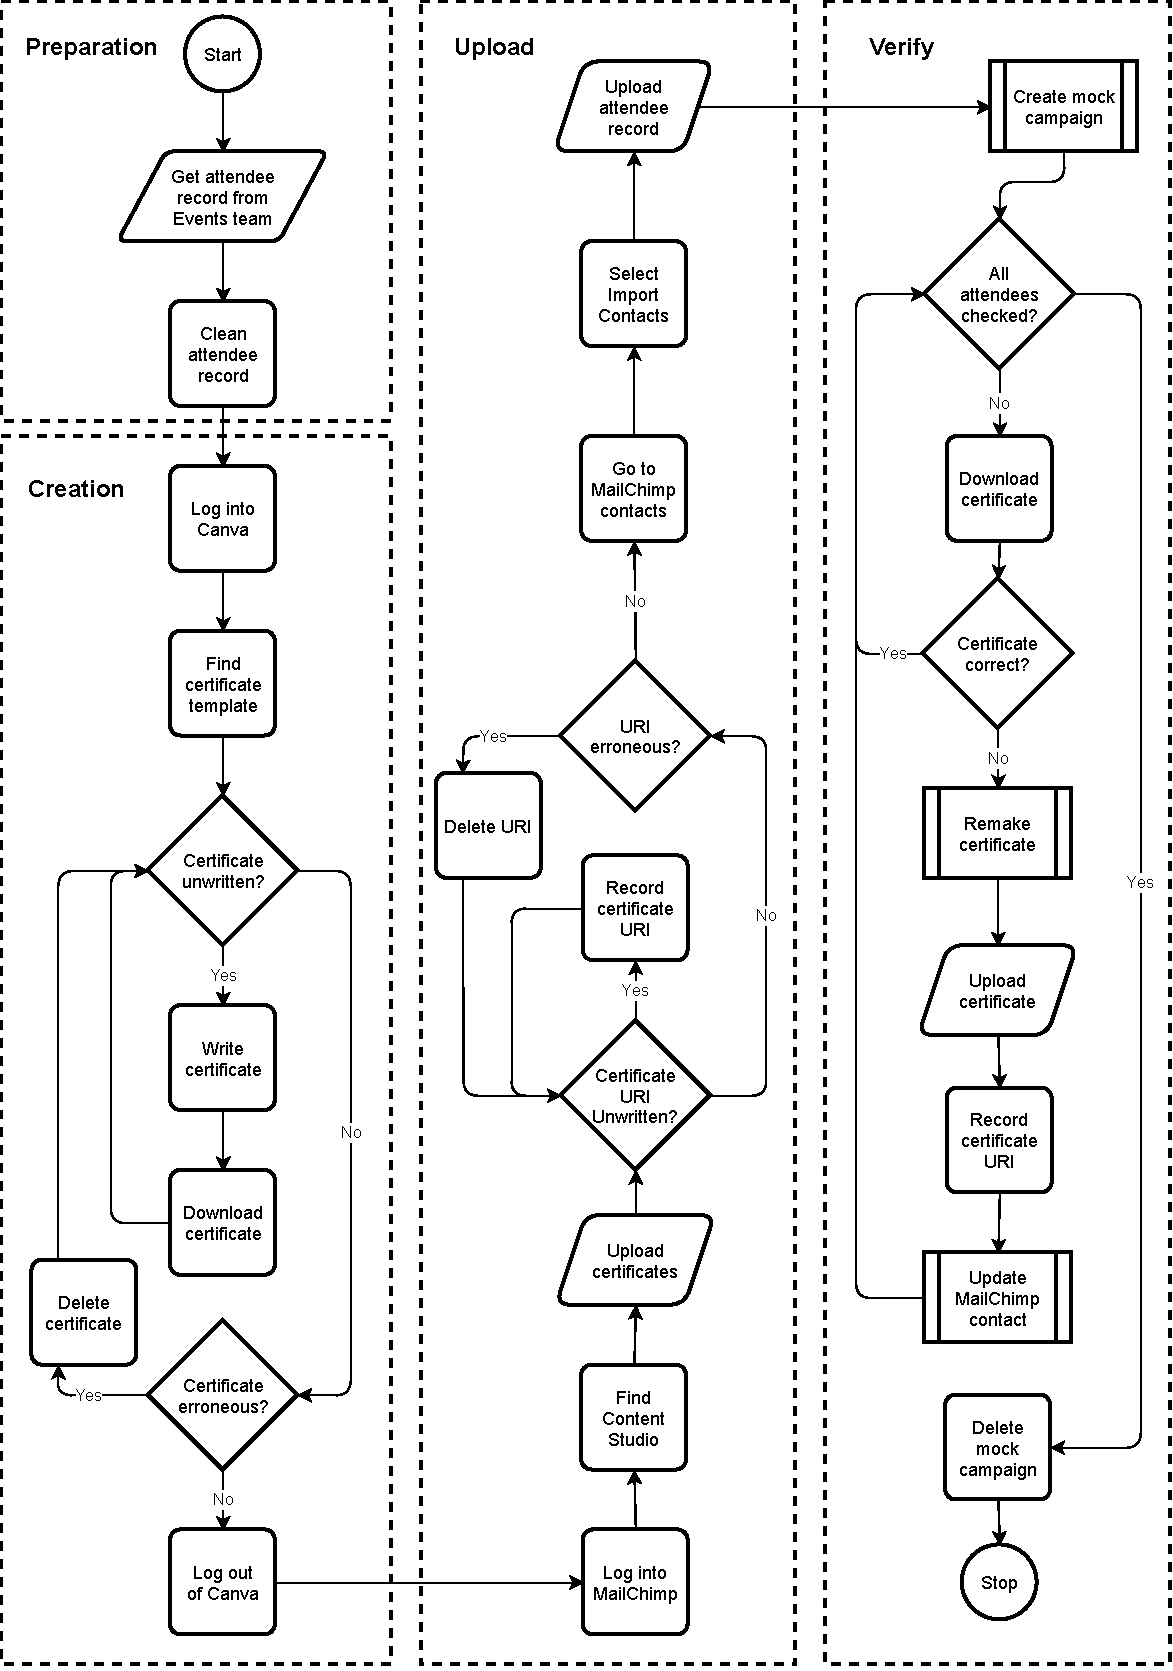
\includegraphics[width=\textwidth]{figures/old_solution.pdf}
    \caption{Old solution flowchart.}
    \label{fig:old-solution}
\end{figure}

\newpage

\section{Solution Overview}

\subsection{Rundown}

After some research, it has been discovered that stages 2, 3, and 4 of the old solution can be automated. For stage 1, instead of logging into Canva and creating each certificate manually, the template can be downloaded once and used to automatically create every certificate. The MailChimp API can be used to automatstage 3, where each certificate can be uploaded and have its URI recorded. With the URIs known, the attendee record can be updated and uploaded to MailChimp. Since the certificates were created automatically, stage 4 becomes redundant. This process is sumarised in figure \ref{fig:new-solution}. With such a script, CIET can be confident in its ability to deliver the correct certificates to its members on time and without significant human time investments.

\begin{figure}[b!]
    \centering
    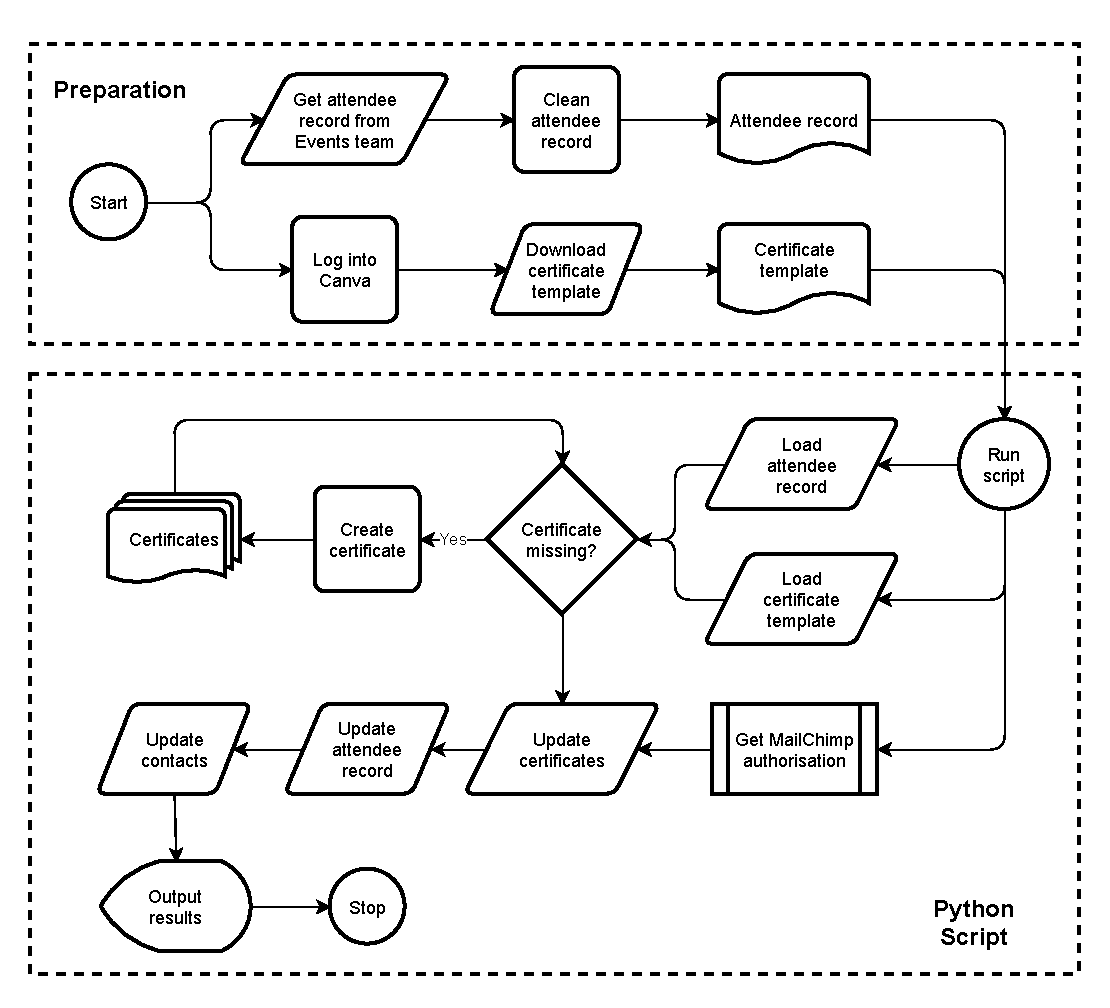
\includegraphics[width=0.8\textwidth]{figures/new_solution.pdf}
    \caption{New solution flowchart.}
    \label{fig:new-solution}
\end{figure}

Realising this goal, however, will require a well organised team and a plan. Due to the various actions this script must perform, a moderately large codebase utilising several libraries and protocols is needed, demanding a significant time investment and expertise. This complexity is compounded by delegating the workload between a team, needing appropriate version control, task management, and enforeable coding standards. Furthermore, such a project could easily suffer from scope creep, especially with the user interface. Hence, the need for subsequent sections in this document to eliminate these issues.

\subsection{Prototype}

For the sake of time, a prototype can be implemented before scope creep becomes an issue. A prototype must include:

\begin{enumerate}
    \item Command line interface to run program.
    \item Must start program with certificate template path, attendee record path, and Mailchimp API and server keys as command line arguments
    \begin{enumerate}
        \item Strongly recommended to use \mintinline{python}{argparse} library.
    \end{enumerate}
    \item Generate a certificate of attendance for each attendee
    \begin{enumerate}
        \item Must be saved into a folder called \mintinline{console}{/certificates} in the current working directory.
        \item Each certificate must be named based on attendee's full name.
    \end{enumerate}
    \item Upload certificates to Mailchimp, keeping track of the file URIs.
    \begin{enumerate}
        \item Uploading of certificates must be done as a batch, not individually uploaded.
    \end{enumerate}
    \item Update the attendee record with the certificate URIs.
    \item Update the Mailchimp contacts with file URIs.
    \item Inform the user of what the program is currently doing.
    \begin{enumerate}
        \item Can just be a simple sentence, e.g. "Uploading certificates to Mailchimp..."
    \end{enumerate}
    \item Be able to process errors without crashing.
    \item Must be able to continue processing certificates when one fails.
    \item Must inform user of which step or certificates failed and why.
    \begin{enumerate}
        \item Can be done once the program has finished everything else.
    \end{enumerate}
    \item Must be able to run on Windows, Linux, and Mac systems capable of running Python 3.
\end{enumerate}

\noindent
For the sake of time and simplicity, the following assumptions can be made:

\begin{enumerate}
    \item The certificate of attendance is known.
    \begin{enumerate}
        \item The only field to be changed is the attendee name.
        \item The exact location of the attendee name field is known and constant.
        \item The placeholder text of the attendee name field is known and constant.
        \item The certificate is always valid.
    \end{enumerate}
    \item The attendee record contains no errors.
\end{enumerate}

\subsection{Minimal Viable Product}

Once a prototype is complete, a minimal viable product (MVP) can be written. The MVP has all the criteria of the prototype, excluding 2, and

\begin{enumerate}
    \item Can be run via an executable.
    \begin{enumerate}
        \item No command line interfacing should be necessary.
    \end{enumerate}
    \item Should have a simple and initiative GUI.
    \begin{enumerate}
        \item GUI does not need to be aesthetically pleasing.
    \end{enumerate}
    \item Can select input files via file explorer.
    \item Must log at least info, warning, error, and critical messages to a log file.
    \begin{enumerate}
        \item Debug messages are optional.
        \item It must be known where the log file is.
        \item The GUI should have a button for viewing the log file.
        \item Strongly recommended to use the \mintinline{python}{logging} library.
    \end{enumerate}
    \item Must use OAuth 2 to get Mailchimp authorisation.
    \begin{enumerate}
        \item The program should not have the option to use API keys.
    \end{enumerate}
    \item Should be able to inform the user of errors that occur in real time without interrupting background tasks.
    \item Use appropriate colour coding and symbols to inform user of successes, warnings, and errors.
    \item Must be able to instantly respond to user inputs without stuttering.
    \item Multiprocessing and multithreading must be used to prevent the program from locking.
    \item Must be able to check attendee record for errors.
    \begin{enumerate}
        \item Repeated email addresses.
        \item Missing names or emails.
        \item Missing required fields.
    \end{enumerate}
    \item Must be able to edit PDF document in GUI.
    \begin{enumerate}
        \item Must be able to view PDF document within GUI.
        \item Must be able to select the field where the full name goes.
    \end{enumerate}
\end{enumerate}

\subsection{Competitive Product}

If the MVP is done, a competitive, market ready, version can be done. This version should have everything the MVP has, and

\begin{enumerate}
    \item Has ultra-specific error messages.
    \begin{enumerate}
        \item Informs the user of what exaclty went wrong.
        \item Where possible, offers a solution.
        \item Where possible, offers links to online documentation.
    \end{enumerate}
    \item Must include install wizard with a build machine.
    \begin{enumerate}
        \item Must be able to choose where to install program.
    \end{enumerate}
    \item Allows user to select where log files are saved.
    \item Allows user to select what types of messages get logged.
    \item Must be able to select multiple fields in template as placeholders.
    \begin{enumerate}
        \item Must be able to select what each placeholder gets replaced with graphically.
        \item Must be able to select between attendee attribute, constant value (e.g. event name), or system value (e.g. timestamp).
    \end{enumerate}
    \item Must be able to generate PDF report of what happened.
    \begin{enumerate}
        \item Can select where report gets saved to.
        \item Can select what goes on the report.
    \end{enumerate}
    \item Must have an aesthetically pleasing GUI.
\end{enumerate}

\newpage

\section{Prerequisite Knowledge}

\subsection{Python Language}

While Python was originally designed as a simple scripting language, it has since evolved into one of the most used and popular languages. The simplicity of Python lends itself well to rapid prototyping, so simple that Python's syntax is often considered to be pseudocode. Furthermore, the library support for Python, both first and third-party, makes it extremely easy to make complex tasks simple. The sheer abundance of libaries available creates a compunding effect, as existing libraries makes it easier to wrote other libraries, leading to an exponential growth in library support. Whenever a new protocol or standard becomes prominent, chances are someone has already made a Python library to make it trivial to implement the protocol or standard within other programs. Additionally, the popularity of Python means there is ambundant support online for both known issues and asking online for assistance. For the sake of prototyping, it is difficult to find a better language than Python.

Considering the ambundance of support for Python, learning the language is best done with interactive tutorials foudn online. Such examples include W3 Schools, Codecademny, and Learn Python. Numerous other tutorials exist, such as those on Tutorials Point and the countless YouTube videos; however, these tutorials lack an interactive component, leading to reading or watching without learning. When learning a new language, the source is less important than the interaction between the material and the student.

Where Python's weakness lies is in its performance. Since Python is a weak typed language, datatype checking must be done during runtime, greatly reducing performance. Far worse, the interpreted nature of Python means compiler optimisations cannot be performed, slowing down Python to a crawl. Compared to optimised compiled languages, such as C, Rust, and C++, Python performs dozens of times worse when comparing equivelant programs. This can be greatly mitigated by taking advantage of scientific libraries, such as NumPy and Pandas. These libraries are written in C and C++, allowing for speeds within the ballpark of C, C++, and Rust. However, certain conventions must be followed to take advantage of vectorised data, leading to data needing to be structured in vectors or matrices. Unfortunately, this will only result in a performance increase when doing mathematical operations on numeric data, such as vector dot products or summing an array. Ergo, Python is a poor choice for performance critical applications.


\subsection{OSI and TCP/IP Models}

To understand how programs interface with each other over the internet, the Open Systems Interconnection (OSI) model must be introduced. Starting in the late 1970s, the OSI model details how computers, or ``nodes'', communicate with each other over a network. The model is split into seven layers, each with their own purpose and protocols, shown in table \ref{table:OSI-model}. Each layer only needs to know about the adjacent layers, decoupling the responsibilities as much as possible. When sending messages over a network, the sender goes through the layers from top-to-bottom, whereas the receiver goes the layers bottom-to-top. Despite the significant learning curve, the OSI model successfully delegates the numerous responsibilities of network communication across seven mostly decoupled layers.

\begin{table}[t!]
    \begin{threeparttable}[t]
        \caption{OSI Model for computer networking}
        \label{table:OSI-model}
        \begin{tabular}{m{0.1\textwidth}<{\centering} || m{0.3\textwidth} | m{0.3\textwidth} | m{0.3\textwidth}}
            \toprule
            \textbf{No.}    &   \textbf{TCP/IP Model} &   \textbf{OSI Model}  &   \textbf{Protocols} \\
            \midrule
            7   &   \multirow{3}*{Application}      &   Application     &   HTTP, FTP, WS, RTP \\
            6   &                                   &   Presentation    &   JPEG, TSL, SSL \\
            5   &                                   &   Session         &   NFS, SQL, PAP \\
            \hline
            4   &   Host-to-Host                    &   Transport       &   TCP, UDP \\
            \hline
            3   &   Internet                        &   Network         &   IPv4, IPv6 \\
            \hline
            2   &   \multirow{2}*{Network Access}   &   Data Link       &   ARP, CDP, STP \\
            1   &                                   &   Physical        &   Ethernet, Wi-Fi \\
            \bottomrule
        \end{tabular}
    \end{threeparttable}
\end{table}

{\setlength{\parindent}{0cm}
\vspace{\baselineskip}
\textbf{1. Physical Layer}

What physical devices are used to connect the nodes within a local area network (LAN). By extension, also dictates the bit rate, what receives data, and what sends data. Does not understand data beyond a sequence of 1s and 0s.

\vspace{\baselineskip}
\textbf{2. Data Link Layer}

Establishes and terminates a connection between two physically connected nodes. Data is broken into packets and organised into frames. Uses a logical link control (LLC) to identify network protocols, check for errors, and synchronise frames. Also uses Media Access Control (MAC) addresses to uniquely identify nodes and setup connections, including permissions.

\vspace{\baselineskip}
\textbf{3. Network Layer}

Uses routers to sent segment of data from layer 4 and pair them with an address, typically an IPv4 address. Each segment with sent between routers to the correct LAN, where layer 2 takes control. By extension, also responsible for determining the fastest path to sent the segments through routers. Without layer 3, communication between LANs (e.g. the entire internet) would not be possible. Sometimes known as a ``connectionless'' protocol, as messages are sent without checking they were successfully sent.

\vspace{\baselineskip}
\textbf{4. Transport Layer}

Takes data being sent from layer 5 and breaks it into segments to be sent over layer 3. Also responsible for reassembling segments back into the full message on the receiving end. Transmission Control Protocol (TCP) prioritises reliability over speed, ensuring that segments (called packets) are received intact. If a segment is curropt or not sent within a time limit, the receiver asks for the segment again. The receiver must also sent back a message. If the response is incorrect, the sender resends the message. Alternatively, User Datagram Protocol (UDP) treats segements as datagrams, sending them without any error checking, prioritising speed over reliability. Just like layer 3, UDP is also known as connectionless. The former is used for internet browsing and uploading to a server, whereas the latter is used for streaming videos, music, and playing games online.

\vspace{\baselineskip}
\textbf{5. Session Layer}

Manages communication channels, or ``sessions'', between devices. Responsible for opening sessions, ensuring sessions remain open during data transfer, and closing sessions. Can also setup ``checkpoints'', ensuring that if the data flow is interrupted, it can be continued latter without restarting.

\vspace{\baselineskip}
\textbf{6. Presentation Layer}

Prepares data from layer 7 before being sent via layer 5. Performs compression, encoding on the sending end, decoding on the receiving end, and encryption. The `s' in ``https'' stand for secure and is handled by the Transport Layer Security (TLS) protocol, often mistaken for the outdated and hacked Secure Socket Layer (SSL).

\vspace{\baselineskip}
\textbf{7. Application Layer}

The programs that are generating the data being sent and received. Examples include web browers, email clients, servers, and streaming services such as Netflix and Twitch. Also responsible for presenting the data in a meaningful way to end users.
}

\vspace{\baselineskip}

The observant reader would also notice that there is a simplified TCP/IP model, only comprised of four layers. In it, the bottom two layers of OSI are combined into the Network layer, where frames are transmitted between nodes on a LAN via mapping IP addresses and port numbers to MAC addresses. The next layer, called the ``Internet layer'', uses the assigned IP addresses to direct packets to the correct LAN. The internet layer also uses Internet Control Message Protocol (ICMP) to inform hosts about network issues, encapsulated within the IP dataframes. To determine the physical address of a node, layer 2 also uses Address Resolution Protocol (ARP). Layer 3 in the TCP/IP model is identical to the transport layer in the OSI model.\footnote{Despite the name, UDP can be used in the TCP/IP model} Lastly, the top three layers of OSI are combined into the application layer in TCP/IP model. Due to the reduced complexity, the TCP/IP model is often used over the OSI model for internet communications.


\subsection{HTTP Requests and Responses}

Of interest to interfacing with internet-based servers is the hypertext transfer protocol (HTTP). Invented circa 1990, HTTP is a request-response protocol, transferring data in simple text documents. As of the time of writing, HTTP 1.1 is the most commonly used version, with 2.0 slowly replacing 1.1. In all versions, the first step is for the client to connect to the server via a TCP handshake. Once a connection has been established, the client can proceed to send a ``request'', which the server processes then replies with a ``response''.

The request is a text document made of three, sometimes four parts. The first line is always the request header, formatted as the method type, followed by the path to the resource, then the HTTP version. Afterwards, each line then comprises the one key-value pair of the header, used to specify metadata, such as the host, accepted languages, authorisation codes, connection type, and expected content type(s). To end the header, an empty line must then follow. For some requests, a body may also be necessary, such as the content being uploaded to the server. Below is an example of such a request.

\vspace{0.5\baselineskip}

\inputminted[linenos=true]{html}{http_examples/post_request.html}

Once the server has finished processing the request, it sends back a response, formatted very similarly to a request. The response's first line is always the status line, formatted as the HTTP version, the status code, then the status message. The status code is a three digit code informing the client of how the server handled the request. The first digit is the broad type of code, then the next two digits specifies the exact type of code. The status message is simply a humanly readable message version of the status code. After the status line, the header fields are then declared line-by-line, ending with an empty line. For some requests, a body will also be included after the empty line. See the example below.

\vspace{0.5\baselineskip}

\inputminted[linenos=true]{html}{http_examples/get_response.html}

\begin{info}[HTTP Status Codes]
For long messages split into multiple requests, a \texttt{1xx} status code means the server successfully received the segement and the client should send the next. \texttt{2xx} means the message was received, uinderstood, and processed successfully. \texttt{3xx} means the server does not have the resource being requested but does know another server that does.\footnote{Responses with status codes of \texttt{3xx} should always include the server connection details in the body} 4xx means the client did something wrong, such as the classis \texttt{404} file not found error. Lastly, \texttt{5xx} means the server did something wrong.
\end{info}

As of HTTP 1.1, there are nine accepted methods. Introduced in HTTP 0.9 (the firt public version), the \texttt{GET} request is a simple read only request to retrieve a copy of a resource from the server. As of HTTP 1.0, the \texttt{POST} request allows for clients to upload new resources onto the server. Also as of HTTP 1.0, the \texttt{HEAD} request works identically to a \texttt{GET} request, expect that the body is not returned. When HTTP 1.1 was made available, two important methods were added: A \texttt{PUT} request allows a client to replace an existing resource on a server with the one in the request body, whereas a \texttt{DELETE} request simply tells the server to delete the specified resource. Similar to a \texttt{PUT} request, a \texttt{PATCH} request tells the server to partially update a resource instead of replacing it. While not commonly used, HTTP 1.1 also introduced the \texttt{TRACE} and \texttt{OPTIONS} request types. The former performs a message loop-back test from the path of the specified resource, whereas the latter requests the server to describe all available commincation options for the specified resource. Lastly, the \texttt{CONNECT} request allows clients to connect to a server through another server, useful for setting up proxy servers or websites using TSL (i.e. HTTPS).

While HTTP 1.1 remains the predominant version as of the time of writing, HTTP 2.0 will eventually replace it. HTTP 1.1 introduced vast performance improvements over 1.0, most notably the ability to remain connected to the server after each request-response cycle instead of having to reconnect to the server. However, in 1.1, the server can only process one request from any client at a time, meaning the client must wait until the current request has been responded before sending another. This has changed in 2.0, allowing for mutliple requests to be sent, processed, and responded to after a connection has been established, shown in figure \ref{fig:http-visualised}. For now, this project can ignore HTTP 2.0, but future versions may need to consider the inevitable obsoletion of HTTP 1.1.

\begin{figure}[h!]
    \centering
    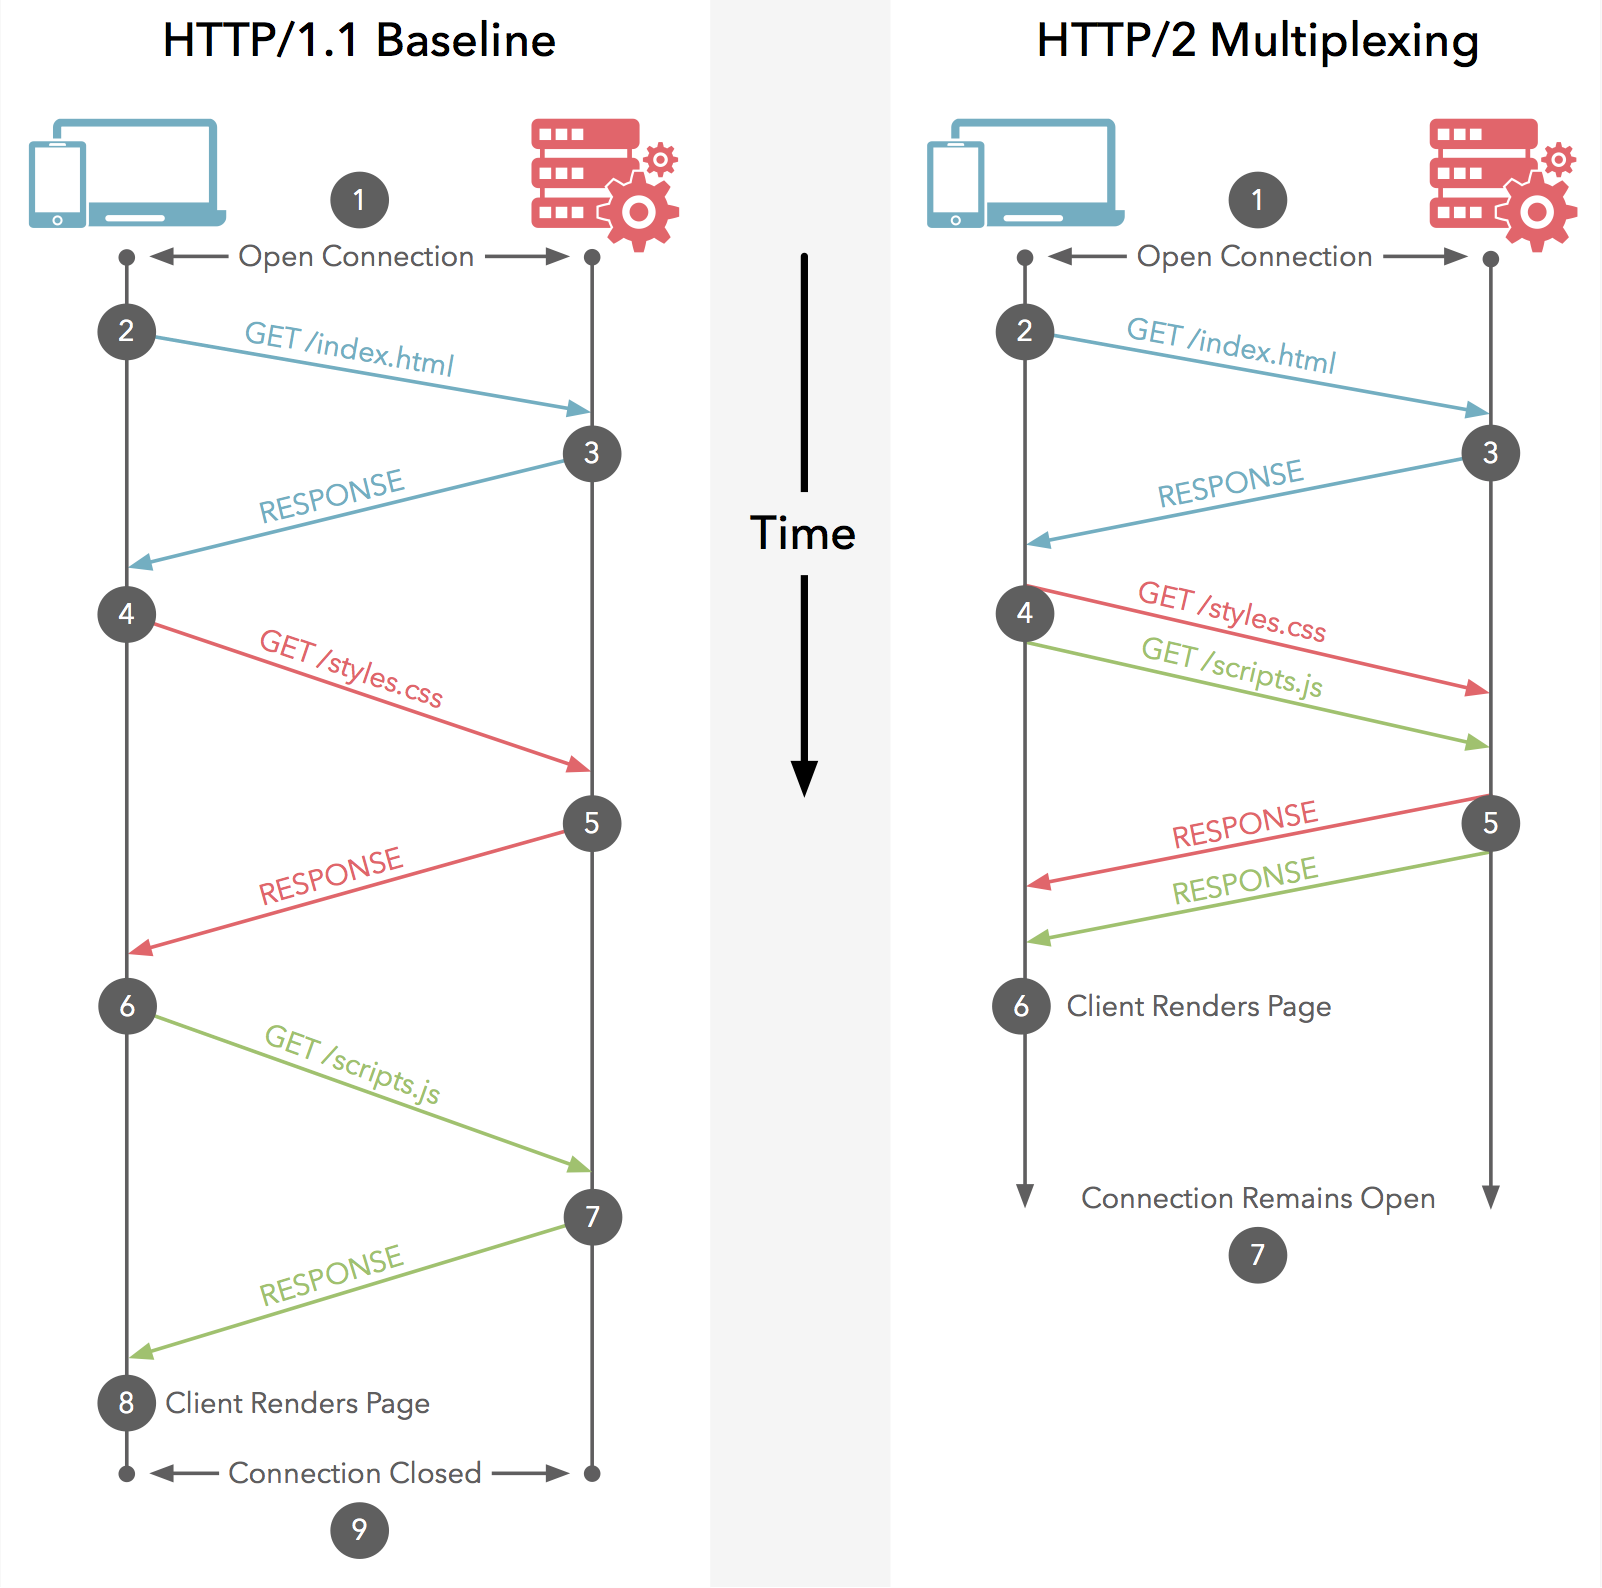
\includegraphics[width=0.8\textwidth]{figures/http1-vs-http2-multiplexing.png}
    \caption{HTTP 1.1 and HTTP 2.0 visualised, with time being directed downwards.}
    \label{fig:http-visualised}
\end{figure}

\subsection{Object Orientation}

Critical to software engineering, object orientated programming (OOP) has proven invaluable to large scale and collaborative code-based projects. This is possible via a sophisticated application of the broad divide and conquer approach, splitting complex programs into simple and decoupled modules and submodules. OOP achieves this through four main principles: encapsulation, abstraction, inheritance, and polymorphism.

\subsubsection{Encapsulation}

Consider the logistics in running a store: the stock available, the stock reserved for customers yet to buy them, preorders, cancellations, the stock on its way, the customers who have signed up as members, newsletters, purchases, overhead costs, etc. How does a business maintain such logistics? Who records the data? Who files and organises the data? WHo has access to what data? Who is authorised to fix errors in the data and what process must they go through to make these fixes? Perhaps msot importantly, who or what ensures the data is valid \textit{before} it is placed with exisitng data? Such problems can be at least mitigated using the OOP paradigm.

Since objects contain data as variables, the objects can be made responsible for protecting the data from curroption. Instead of making the variables directly accessible, the object can have getters and setters (also known as mutators) to access the data. Getters should always return a copy of the variable, whereas getters must validate the new value before setting the variable. For example, it is impossible for a jar to have a negative number of marbles, hence if outside code attempts to remove more marbles from a jar object than what is available an error can be raised and the jar's number of marbles remains unchanged. Similarly, the jar will probably also have a capacity, so that if too many marbles are attempted to be inserted a different error should be raised. Some object variable may not even have getters, such as the length of a collection (e.g. an array or a linked list). Instead, the length variable should automatically change as elements are inserted or removed. Even further encapsulated, other variables may not even have getters, as they may be variables that should only be used by the object internally, such as an array inside of a hash table. Protecting data like this greatly mitigates the data from being curropted or otherwise useless.

\begin{figure}[b!]
    \centering
    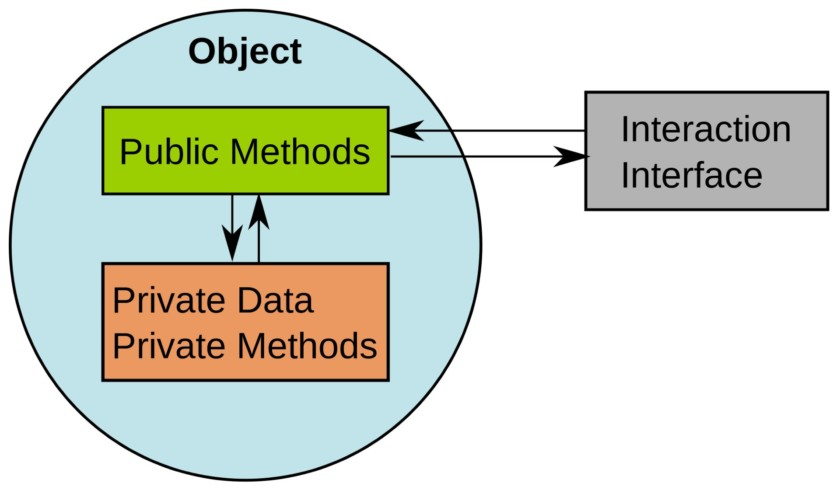
\includegraphics[width=0.6\textwidth]{figures/encapsulation.jpg}
    \caption{Encapsulation visualisation.}
    \label{fig:encapsulation}
\end{figure}

\subsubsection{Abstraction}

As a program become more and more complex, it becomes increasingly difficult to manage the functionality of the program. Trying to track where the functions of a program are organised and located turns inpractical. Even trying to determine if a function has been implemented becomes time consuming and infeasible. This can be partially mitigated by organising functions into thematically narrow and consistent libraries; however, even this approach leads to too many functions to keep track of what has and has not been implemented. For complex programs, especailly those requiring extensive interaction with other programs, a smarter approach is needed.

Abstraction attempts to solve this issue by hiding functionality within objects. Abstraction is simply the process of hiding the implementation by only exposing what the object can do. Hence, outside code only needs to concern itself with what the object can do and not how it does it. Since objects can contain other objects, complex tasks involving several steps using numerous variables can be split accross a tree-like hierarchy of objects. Consider the OSI or TCP/IP model detailed above: with OOP all that is needed is a single \texttt{NetworkManager} that handles how an application sends and receives data without code outside the \texttt{NetworkManager} needing to know about layers below the application layer. Therefore, outside code only needs to call a single method of one object and let it handle how the task is completed.

\subsubsection{Inheritance}

When similar entities need to be modelled, code repitition becomes an issue. Consider a pet tracker for a vetenary that needs to store various types of pets. Obviously, snakes and rabbits are two very different animals that require very different code to model. However, cats and dogs are similar enough that the code modelling these pets would at least somewhat repeat. Repeated code makes it more difficult to maintain, as each repeat must be individually tested, debugged, and modified due to changing environments or requirements, leading to the risk of some repeats not being debugged or changed properly. By extension, this also makes testing more expensive, time-consuming, and error-prone, as each repeat code block being tested will lead to repeat test cases. Clearly, such repitition needs to be eliminated.

\begin{figure}[b!]
    \centering
    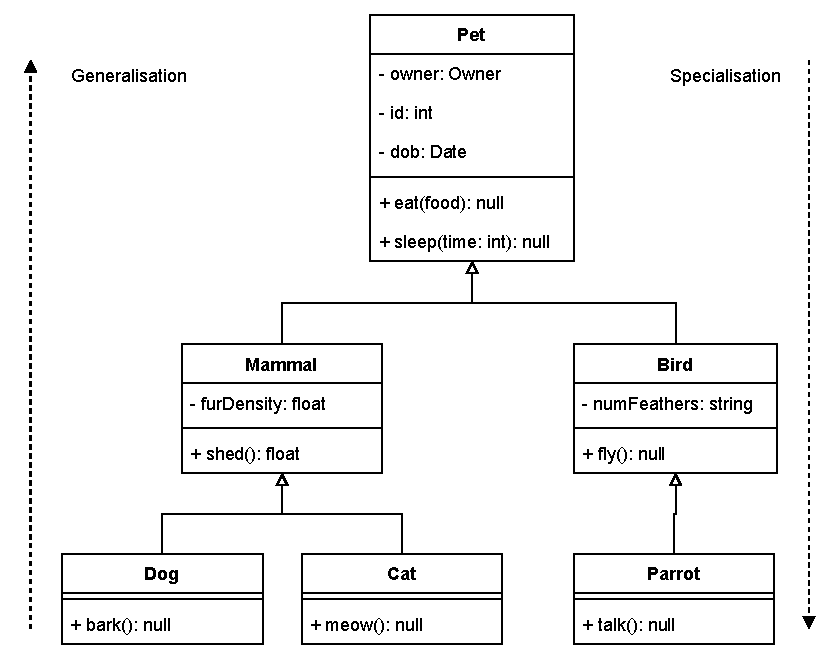
\includegraphics[width=0.7\textwidth]{figures/inheritance.pdf}
    \caption{Inheritance UML example.}
    \label{fig:inheritance-uml}
\end{figure}

OOP programming provides such a solution in the form of inheritance. Simply put, inheritance is the ability of some classes to inherit the code of other classes. For the pet tracker example, a base class called \texttt{Pet} or \texttt{Animal} can be made that contains code common to all pets. E.g., values like owner, pet ID, and date of birth. Further classes can be written that eliminate code repitition for groups of types of pets, e.g. \texttt{Mammal}, \texttt{Reptilian}, \texttt{Bird}, and \texttt{Amphibian}, each of which should inherit from the \texttt{Pet} base class. Then, more specific pet types can be written that inherit from these broad pet types, such as \texttt{Dog}, \texttt{Cat}, \texttt{Turtle}, \texttt{Snake}, \texttt{Parrot}, and \texttt{Frog}. Such inheritance is known as the \textit{is-a} relationship, as a dog \textit{is a} Mammal, which \textit{is a} animal. Designing a codebase like this completely eliminates repetitive functions, greatly speading up the process of writing the codebase and simplifying test cases.

\noindent
\begin{minipage}[t]{0.5\textwidth}
    \vspace{0pt}
    \, Additionally, inheritance also covers one object being contained within another. This type of relationship is known as the \textit{has-a} relationship or association. For example, a car is \textit{not} a type of steering wheel and vice-versa. However, a car \textit{has a} steering wheel. Consider a car manufacturer that needs to design and manufacture cars. While different car models are not identical, they may share identical steering wheels, gearboxes, transmission systems, fuel tanks, wheels, or seats, among other numerous parts. Hence, these identicial parts can be written, tested, and debugged once, then shared across the different car classes. This type of association is known as composition, as the car fully owns the parts it is made of. If the car object is destroyed, the car parts are also destroyed. This is opposed to aggregation, in which the child object can exist independtly of the parent class, such as the cars and the manufacturer. As with the \textit{is-a} relationship, association greatly reduces code repitition.
\end{minipage}
\begin{minipage}[t]{0.5\textwidth}
    \vspace{0pt}
    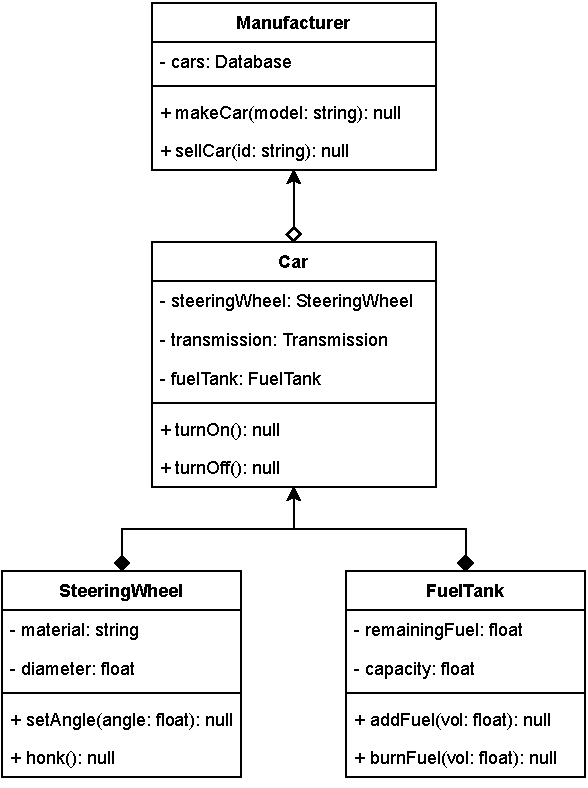
\includegraphics[width=\textwidth]{figures/association.pdf}
    \captionof{figure}{Assocation UML example.}
    \label{fig:association-uml}
\end{minipage}

\subsubsection{Polymorphism}

When developing a codebase, it occansionally becomes useful to have multiple functions or methods that are named the same but perform differently. In \texttt{C}, the \texttt{math.h} library contains functions for finding the absolute value of a number. There are actually two of these functions: the \mintinline{c}{abs()} function and the \mintinline{c}{fabs()} function. The reasoning being is that \mintinline{c}{abs()} takes in an integer whereas \mintinline{c}{fabs()} takes in a double. Since \texttt{C} is a strong typed language with no polymorphism, this practice of having multiple functions perform essentailly the same task becomes inevitable. Even more complicated, consider the case of calculating the area of a shape. Since the areas of shapes are calculated differently from shape to shape, in \texttt{C} there would be one function per type of shape. E.g. \mintinline{c}{circleArea()}, \mintinline{c}{rectArea()}, \mintinline{c}{triangleArea()}, etc. As program requirements start involving extremely similar functions and datatypes, the number of near-identical functions to keep track of becomes inpractical.

Polymorphism solves this issue by allowing multiple functions to share the same name. One such manner of doing so is called ``method overloading'': allowing for a class or object to have multiple methods with the same name but different parameter lists in terms of their datatypes. In Python, this is actually not possible since the datatypes of variables does not have to be declared. Instead, Python achieves pseudo-overloading by allowing for a parameter to have one of multiple valid datatypes (such as \texttt{num} being either an \mintinline{python}{int} or an \mintinline{python}{float}) or by having parameters with default values. Further still, a function in Python can have an optional list of miscellaneous, unnamed parameters and another optional dictionary of named parameters. For example, the Python function

\begin{minted}{python}
def formatNumbers(num, *args, precision=2, **kwargs):
    ...
\end{minted}

\noindent
must be called with a number, but can allow multiple arbitrary numbers to be formated via the \mintinline{python}{*args} list, optionally specify the precision to format the numbers to (defaults to 2 decimal places), and also be called with arbitrary named parameters that are stored inside the \mintinline{python}{**kwargs} dictionary (short for ``keyword arguments'').

Using the \textit{is-a} inheritance principle, it is also possible to achieve polymorphism via ``method overriding''. Going back to the area of shapes example, we can calculate the areas of different shapes without needing multiple methods with different names. Instead, a base class \texttt{Shape} can be written, that has the method \texttt{calcArea()}. This method is known as an ``abstract method'' since it has not been implemented, meaning the \texttt{Shape} class is also abstract. Abstract classes cannot be instantiated into objects, making them useless by themselves. Instead, subclasses of the \texttt{Shape} class can be written that implement this abstract method, such as \texttt{Circle}, \texttt{Rectangle}, and \texttt{Triangle}. The significane of which means that outside code does not need to concern itself with what exact type of shape a \texttt{Shape} object is, only that is has a \texttt{calcArea()} method. Hence, functions can be written once for any arbitrary shape object and more shape types can be written latter without having to change any of these functions.

\subsection{Application Programming Interface}

The world of modern software development is one heavily comprised of using code and services created by third-party organisations or individuals. This is an inevitable consequence of the daunting product requirements that modern software must abide by to remain competitive. However, the pitfalls of using third party services quickly become apparent: \textit{How do we know future changes won't break our code? Will our application still work when this service changes? What security flaws or exploits are exposed allowing others to use our service? What do we do if a third party service does not allow us to access their service via code?} Consider the need for a music editing mobile app that can use music owned by the user from their Spotify, Google Music, Bandcamp, or Apple Music accounts. How does a development team even begin to integrate these services their mobile app?

Solving these concerns introduces the need for Application Programming Interfaces, or APIs. An API, simply put, is a set of commands a program can use to access and upload data to another program. They can be as simple as the set of functions and constants within a library to the monolithic 2 billion line of code Google API. Well designed APIs allow external parties to develop their own applications integrating your service without needing to know how the API works, nor what the external application is or does. APIs also greatly mitigate security issues, as APIs can hide the implementation of the service. External developers using an API can also be sure that future changes to the API will not break their application, as API updates come with a version number, signifying if an API change has occurred. If an API change has occurred, the external developers can simply not use the newer version until they have updated their application to use the newer API. Most relevant to this project, the Mailchimp API is the only way a program can access a user's Mailchimp account without hacking the Mailchimp servers. Without this API, the project would not be possible.

\newpage

\section{PDF Editing and Creation}



\newpage

\section{MailChimp Authorisation}

\subsection{Using API and Server Keys}




\subsection{Using OAuth 2.0}



\newpage

\section{Certificate Uploading}




\newpage

\section{Contact Updating}



\newpage

\section{User Interface}

\subsection{Command Line Interface}






\subsection{Desktop GUI}




\newpage

\section{Version Control}

\subsection{What is Git?}



\subsection{Using Github}



\subsection{Recording Library Requirements}



\subsection{Virtual Environments}



\newpage

\section{Coding Standards}

\subsection{Readability and Maintainability}



\subsection{Documentating using Sphinx}



\newpage

%%\printbibliography

\end{document}